\chapter{Résultats}

Une fois mon pipeline d'analyse exécuté, j'obtiens des fichiers annotés contenant des informations sur la position de la mutation, le TFBS associé à cette mutation, l'allèle de référence, l'allèle muté et le caractère de la mutation (\gls{homozygote} ou \gls{heterozygote}). L'analyse bioinformatique de ces informations suivant différents critères comme le nombre de mutations observées dans chaque cas, en fonction de la localisation ou encore les gènes cibles de chaque TFBS, est présentée ci-dessous.

\section{Analyse des mutations somatiques dans les TFBS}

Dans le but de détecter les variants somatiques, j'utilise deux logiciels de détection de variants dans mon pipeline. Je m'intéresse donc à la proportion de variants détectés à la fois par l'un et par l'autre.

Les résultats obtenus pour deux de nos cas (LMS1 et LMS19T1bis) sont présentés sur les diagramme de Venn de la figure \ref{fig:venn}. 

\begin{figure}[h]
\centering
\begin{subfigure}{0.3\textwidth}
\centering
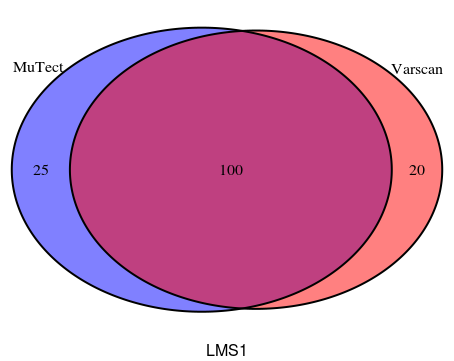
\includegraphics[scale=0.6]{Figures/LMS1.png}
\end{subfigure} 
\hspace{2.5cm}
{\vrule height 3cm width 0.1mm} 
\hspace{1cm}
\begin{subfigure}{0.4\textwidth}
\centering
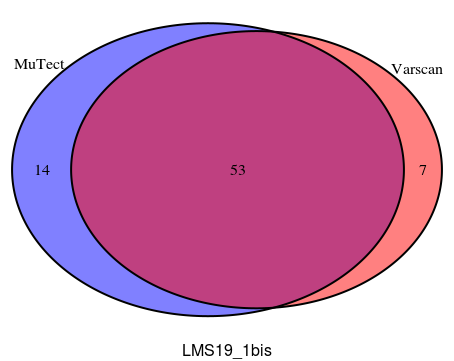
\includegraphics[scale=0.6]{Figures/LMS19_1bis.png}
\end{subfigure}
\captionsetup{justification=centering}
\caption{Nombre de mutations communes à \textbf{MuTect} et \textbf{Varscan} pour 2 échantillons de la cohorte}
\label{fig:venn}
\end{figure}

Le nombre de variants détectés par les deux logiciels varie d'un échantillon à l'autre.  Dans l'exemple de la figure \ref{fig:venn}, pour un total de 125 variations détectées dans le LMS1, 100 sont détectées à la fois par \textbf{MuTect} et par \textbf{Varscan}, soit 66\% du total. Dans le cas du LMS19T1bis, ce taux monte à 72\%.

En moyenne, 84\% des variations sont détectées par les deux logiciels. J'utilise l'intersection des deux résultats pour obtenir les mutations les plus probables.

\newpage

Je formule l'hypothèse que le nombre de mutations ne dépend pas de la localisation tissulaire des tumeurs. L'histogramme \ref{fig:mut} présente le nombre de variations qui ont été détectées et sélectionnées par les deux logiciels pour chacun des cas. 

\begin{figure}[h]
\centering
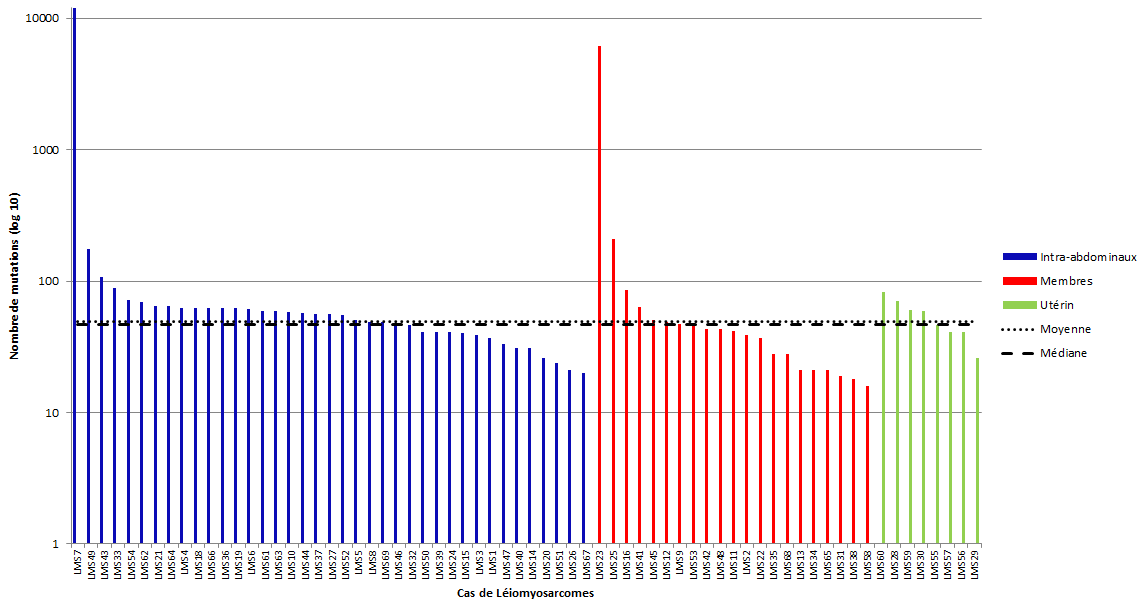
\includegraphics[width=18cm,height=12cm]{Figures/mutations.png}
\captionsetup{justification=centering}
\caption{Nombre de TFBS mutés par cas \\ 
\textit{Cas triés par type de localisation}}
\label{fig:mut}
\end{figure}

Je constate qu'il y a en moyenne 50 mutations par cas de LMS, quelle que soit la localisation. Il ne semble pas y avoir de corrélation entre le nombre de mutations des TFBS et la localisation du LMS, l'hypothèse peut être retenue.

Les cas 7, 23 et 25 se distinguent des autres par un nombre de mutations nettement supérieure à la moyenne (calculée sans ces échantillons). Pour les cas 23 et 25 la majeure partie des mutations sont du type CC$\rightarrow$TT. De telles mutations sont la signature d'une exposition aux UV \citep{signature}. Ces deux échantillons proviennent respectivement du cuir chevelu et du bras, deux zones pouvant être exposées au soleil, c'est pourquoi leurs mutations portent majoritairement la signature des UV.
Le cas 7 ne peut être expliqué par les annotations cliniques actuelles, une étude plus approfondie devra être réalisée.

Pour la suite des analyses, ces trois cas ont été mis de côté car ils représentent des cas particuliers pouvant altérer les résultats statistiques.

Les différents cas analysés ayant été prélevés à différentes localisations, il m'est possible d'étudier l'impact de cette localisation sur le nombre de TFBS mutés pour chacune des trois catégories (Intra-abdominale, Utérine, Membres).

\newpage

Le nombre de mutations des TFBS identifiées dans chaque cas en fonction de la localisation tissulaire de la tumeur est étudié. Les \og boxplots\fg ~de la figure \ref{fig:mut_n} présentent les résultats de cette étude.

\begin{figure}[h]
\centering
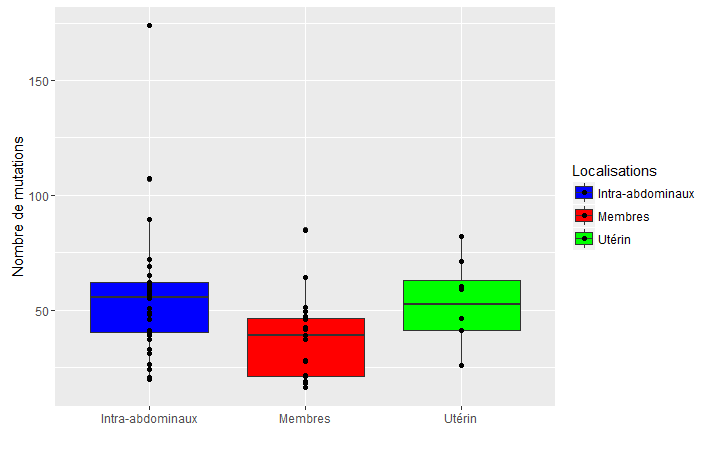
\includegraphics[scale=0.5]{Figures/number_mutations.png} 
    \caption{Variabilité du nombre de mutations en fonction de la localisation} 
    \label{fig:mut_n}
\end{figure} 

Il semble qu'il y a plus de mutations dans les échantillons intra-abdominaux et utérin que dans les membres. Cependant, le nombre de cas est très différent pour chacune des conditions (38 intra-abdominaux, 19 membres et 8 utérins), il est donc difficile de conclure précisément que la localisation de la tumeur a un impact sur le nombre de mutations.

Afin de confirmer les résultats précédents, des tests statistiques sont nécessaires. Ces tests peuvent être paramétriques (ex : t-test) ou non paramétriques (ex : Wilcoxon). Je détermine si l'échantillon suit une loi normale pour savoir quel test réaliser. Les résultats du test de normalité sont présentés sur la figure \ref{fig:shap}. 

\begin{figure}[h]
\centering
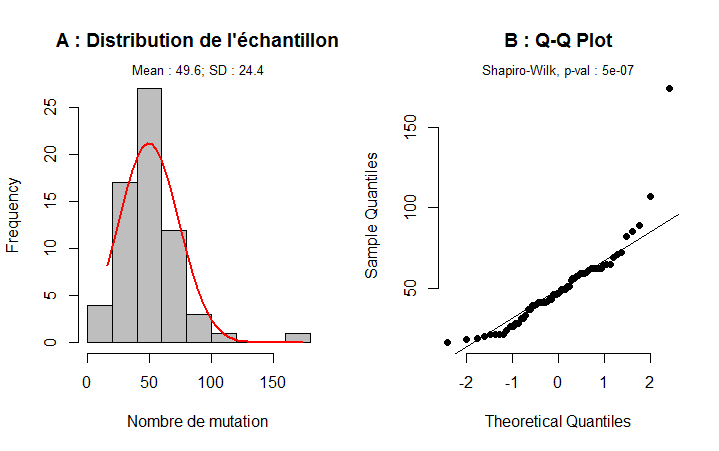
\includegraphics[width=15cm,height=8cm]{Figures/shapiro.png}
\captionsetup{justification=centering}
\caption{Test de normalité \\ 
\textit{A : Répartition du nombre de mutations dans la cohorte, B : Distribution de la cohorte par rapport à la loi normale}}
\label{fig:shap}
\end{figure}

La courbe rouge (\ref{fig:shap}.A) représente la densité de répartition des cas, elle n'est pas Gaussienne donc la population ne suit pas une loi normale. Le diagramme quantiles-quantiles (\ref{fig:shap}.B) montre que la distribution empirique des cas ne corrèle pas celle de la loi normale. De plus, la p-value est significative (p-val = $5E^{-0.7}$), l'hypothèse nulle selon laquelle la population suit une loi normale est rejetée.

Pour déterminer s'il y a une différence significative du nombre de mutations des TFBS entre les localisations, je fais un test de Wilcoxon sur échantillons appariés.

L'hypothèse nulle est qu'il n'y a pas de différence significative entre le nombre de mutations dans les échantillons et la localisation des tumeurs. Le tableau \ref{tab:wilc} contient les p-values obtenues à l'issue du test de Wilcoxon.

\begin{table}[h]
\centering
\begin{tabular}{l|c|c|}
\cline{2-3} & Intra-abdominaux & Membres\\
\hline
\multicolumn{1}{|l|}{Membres} & 0.014 & - \\
\hline
\multicolumn{1}{|l|}{Utérins}  & 0.052 & 0.185 \\
\hline
\end{tabular}
\caption{p-value du test de Wilcoxon}
\label{tab:wilc}
\end{table}

Lorsque je compare l'ensemble des échantillons intra-abdominaux et des membres, la p-value est significative (p-val = 0.014), l'hypothèse nulle est donc rejetée. La localisation des tumeurs a une influence sur le nombre de variations.

Les p-values observées lors de la comparaison des échantillons intra-abdominaux ou membres ou utérins montre  qu'il n'y a pas d'influence de la localisations des tumeurs sur le nombre de variations.

Les analyses statistiques montrent que la localisation peut être corrélée au nombre de mutations des TFBS dans chaque échantillon. La suite de mes analyses portent donc sur le nombre de cas présentant des mutations pour les TFBS de chaque facteur de transcription et ce indépendamment de leur localisation.

\section{Caractérisation des mutations}

Je me suis intéressée aux pourcentages d'échantillons portant des mutations des TFBS pour chacun des facteurs de transcription. La figure \ref{fig:pourcent} présente ces pourcentages. 

\begin{figure}[h]
\centering
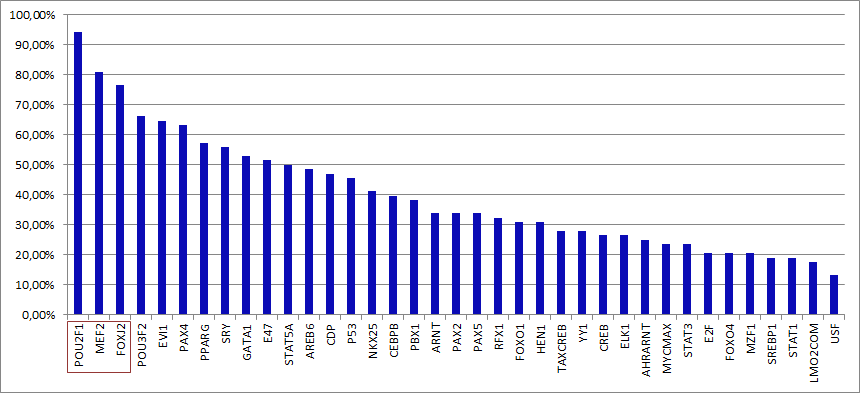
\includegraphics[scale=0.7]{Figures/pourcentage.png}
\captionsetup{justification=centering}
\caption{Pourcentage de cas mutés pour chaque facteur de transcription présentant des TFBS mutés}
\label{fig:pourcent}
\end{figure}

Je constate que les TFBS du facteur de transcription POU2F1 sont mutés dans plus de 90\% des cas, et ceux de MEF2 et de FOXJ2 sont mutés dans plus de 70\% des cas.  Ces trois facteurs de transcription ont respectivement des rôles dans  l'expression du  gène récepteur de la gonadotropine, l'activation de la myogénèse et la migration cellulaire. Des altérations de ces trois facteurs ont été observées dans d'autres cancers. La sur-expression de FOXJ2 diminue la migration cellulaire dans le cancer du sein \citep{foxj2_cancer},la sur ou sous expression de POU2F1 dérégule les fonctions souches des cellules normales et cancéreuses de tous les tissus \citep{oct1_cancer}, la sous-expression de MEF2 entraîne l'augmentation de la prolifération cellulaire \citep{mef2_cancer}. J'ai donc focalisé la suite de mes analyses sur ceux-ci.

Le tableau \ref{fig:tf}, regroupe le nombre de mutations des TFBS pour chacun des trois facteurs de transcription précédemment cités. J'ai sélectionné un échantillon de 6 cas différents de LMS (2 intra-abdominaux, 2 membres et 2 utérins) au hasard parmi les 68. 

\begin{figure}[h]
\renewcommand{\figurename}{Tableau}
\centering
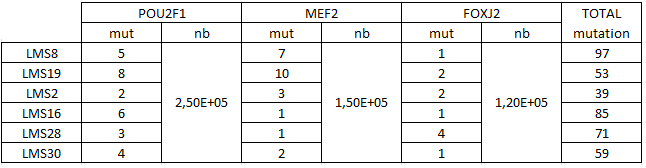
\includegraphics[scale=1]{Figures/table.png}
\captionsetup{justification=centering}
\caption{Nombre de TFBS mutés pour POU2F1, MEF2 et FOXJ2\\
\textit{mut : nombre de mutations, nb : nombre total de TFBS existant pour ce facteur, TOTAL : nombre de TFBS mutés dans l'échantillon}}
\label{fig:tf}
\end{figure}

Je constate que pour chaque cas, il y a en moyenne 4.5 TFBS de POU2F1 mutés dans le même échantillon (4 pour MEF2 et 1.8 pour FOXJ2). 

Ces résultats sont purement prédictifs, des analyses biologiques doivent être réalisées pour les vérifier. J'ai sélectionné trois mutations situées, chacune provenant d'un LMS différent (LMS5,LMS9 et LMS29) et étant placée au milieu du TFBS car lorsque la mutation est située en périphérie elle risque de toucher une autre portion du génome. Ces trois mutations ont été transmises aux biologistes de l'équipe pour une vérification expérimentale.

Cette vérification se déroule en deux étapes. La première est une analyse \og Polymerase Chain Reaction\fg durant laquelle la séquence d'intérêt est amplifiée. La seconde est un séquençage de l'ADN par la méthode Sanger. 

Le résultat de cette analyse pour le LMS5 est présenté sur la figure \ref{fig:oct}.

\begin{figure}[h]
\centering
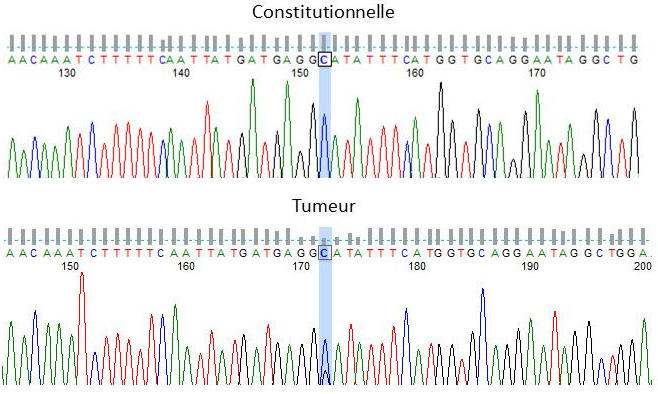
\includegraphics[width=15cm,height=6.5cm]{Figures/OCT1.jpg}
\captionsetup{justification=centering}
\caption{Chromatogramme des séquences d'ADN constitutionnel et tumoral du LMS5
\\ \textit{haut : séquence constitutionnelle, bas : séquence tumorale \\ Bleu : position de la mutation étudiée}}
\label{fig:oct}
\end{figure}

Je constate que sur le \gls{chromatogramme} de la figure \ref{fig:oct} de la séquence tumorale une mutation C $\rightarrow$ G à la position indiquée par les analyses bioinformatiques est présente. Cette mutation est absente de la séquence constitutionnelle, elle peut être caractérisée de somatique.

Sur les trois mutations testées, les analyses biologiques sont revenues positives pour deux échantillons (le LMS5 et le LMS9). Le troisième échantillon (LMS29) présente trop de bruit de fond pour confirmer la présence de la mutation. 

J'ai constaté qu'en moyenne 3 TFBS du même facteur de transcription sont mutés dans le même échantillon (voir tableau \ref{fig:tf}). Il apparaît intéressant d'étudier l'impact de ces mutations sur les gènes cibles des facteurs de transcriptions et plus précisément sur leur expression.

Pour étudier l'expression des gènes cibles des trois facteurs de transcription sélectionnés (POU2F1, MEF2, FOXJ2), j'analyse les valeurs de FPKM pour chacun des gènes situés à proximité de chacun des TFBS mutés.

\begin{figure}[h]
\centering
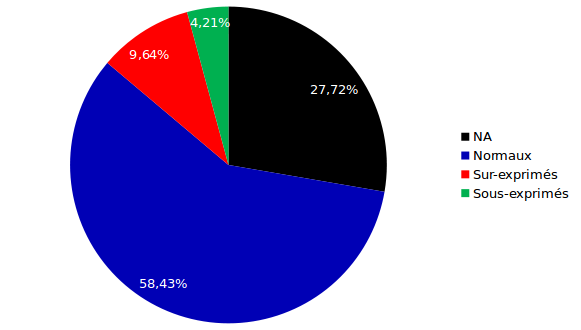
\includegraphics[scale=0.9]{Figures/Camembert.png}
\captionsetup{justification=centering}
\caption{Proportion de gènes sur ou sous exprimés \\ NA : Sans valeur de FPKM}
\label{fig:cam}
\end{figure}

Parmi tous les gènes, j'observe sur le graphique en secteurs (figure \ref{fig:cam}) que 31\% n'ont pas de valeur de FPKM. Ils correspondent à des pseudogènes ou des gènes non-codant, ils ne sont pas présents dans les données de transcriptome qui servent au calcul du FPKM et n'ont donc aucune valeur.

Dans 56\% des cas, les gènes n'ont pas de changement d'expression. Il est possible que ces gènes ne soient pas des cibles du facteur de transcription pour lequel le TFBS est muté ou qu'un autre facteur de transcription compense. Une troisième hypothèse serait qu'un autre facteur de transcription se soit fixé sur le site muté et qu'il joue un rôle similaire sur le même gène.

Parmi les gènes récupérés à proximité des TFBS mutés, seulement 13\% sont sur-exprimés ou sous-exprimés. Parmi ces gènes se trouvent des gènes cibles, il est possible que la différence d'expression de ceux ci soit liée à la mutation du TFBS.

\newpage
Les gènes cibles des facteurs de transcription sont contenus dans deux bases de données (partie \ref{subsec:identification}). L'intersection de cette base avec le fichier des 10 gènes voisins des TFBS me permet de savoir combien de gènes cibles sont présents.

\begin{figure}[h]
\centering
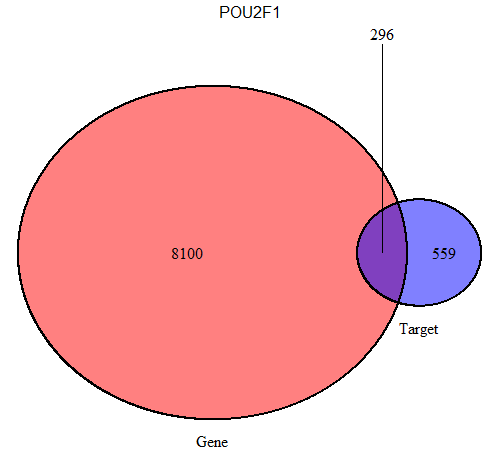
\includegraphics[scale=0.6]{Figures/POU2F1.png}
\captionsetup{justification=centering}
\caption{Nombre de gènes associés aux TFBS mutés de POU2F1 \\ Bleu : gènes cibles identifiés dans \textbf{TRANSFAC}, Rouge : 10 gènes autour de chaque TFBS}
\label{fig:pou}
\end{figure}


Dans le cas du facteur de transcription POU2F1 présenté sur la figure \ref{fig:pou}, je constate que la proportion de gènes cibles présents parmi les gènes voisins des TFBS est de 2\%. J'observe des résultats similaires pour les deux autres facteurs étudiés : MEF2 et FOXJ2.

L'analyse de la figure \ref{fig:cam} m'a permis d'identifier des gènes sur ou sous exprimés autour des TFBS. Sur l'ensemble de ces gènes, certains sont des gènes cibles du facteur de transcription étudié (figure \ref{fig:pou}). Je m'intéresse alors à la proportion de gènes sur ou sous exprimés étant également des gènes cibles.

\begin{figure}[h]
\centering
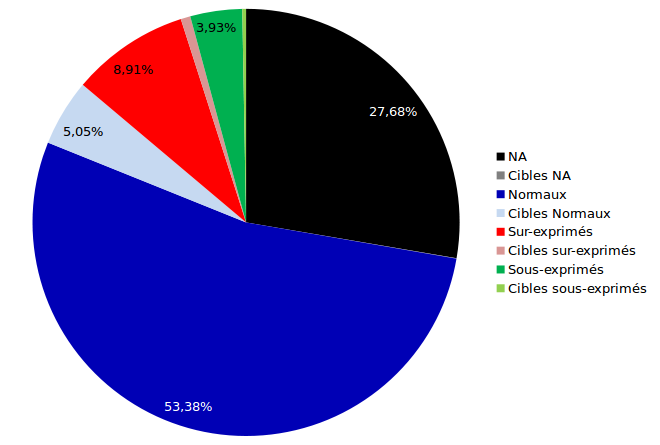
\includegraphics[scale=0.7]{Figures/Cible_expression.png}
\captionsetup{justification=centering}
\caption{Proportion de gènes cibles en fonction de l'expression\\
\textit{Sur tous les TFBS et tous les échantillons}}
\label{fig:pou}
\end{figure}

Parmi tous les gènes proches des TFBS, j'observe que 5.05\% des gènes n'ayant pas de changement d'expression sont des gènes cibles. L'expression des gènes étant régulés par plusieurs facteurs de transcription, il est possible qu'il y ait eu un phénomène de compensation via un autre facteur.

Une faible proportion des gènes sur-exprimés (0.73\%) et des gènes sous-exprimés (0.28\%) sont également des gènes cibles, soit 92 gènes sur les 9169 récupérés autour des TFBS. Dans ces deux cas, il est possible que la mutation du TFBS ait empêcher le bon fonctionnement du facteur de transcription associé.

Les rôles de ces 92 gènes dans le programme transcriptionnel sont variés. Une analyse de l'ontologie de ces gènes (GO) permet de connaître les différents rôles. La figure \ref{fig:go} présente le résultat de cette analyse pour les 20 éléments les plus représentatifs (p-value ajustée Benjamini-Hochberg).

\begin{figure}[h]
\centering
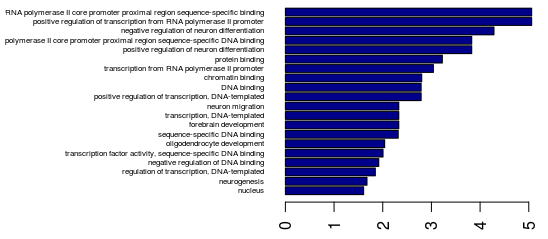
\includegraphics[scale=1]{Figures/GO.png}
\captionsetup{justification=centering}
\caption{Analyse d'enrichissement des gènes cibles de POU2F1, MEF2 et FOXJ2}
\label{fig:go}
\end{figure}

La majeure partie de ces gènes sont impliqués dans les régulations de la transcription au niveau du promoteur de l'ARN polymérase II lequel permet la formation du complexe d'initialisation. D'autres sont impliqués dans la différenciation cellulaire ou la fixation des différents éléments du génome (chromatine, protéine, ADN) ou encore dans la régulation de la différenciation neuronale.

L'hypothèse de départ est que les mutations des TFBS peuvent avoir un impact sur l'expression des gènes cibles des facteurs de transcription qui leurs sont associés. 

L'analyse des TFBS démontre que, quelle que soit la localisation des tumeurs, le nombre de mutations reste le même (en moyenne 50). J'ai également observé que plusieurs TFBS d'un seul facteur de transcription peuvent être mutés dans le même échantillon, ces mutations étant toutes uniques.

L'analyse des gènes proches des TFBS mutés démontre que très peu de ces gènes présentent un changement d'expression. Cependant, parmi tous les gènes récupérés, une partie importante concerne des gènes non codant ou des pseudogènes, il faudra donc refaire les analyses en les intégrant dans l'analyse RNASeq initiale. 

Dans les gènes présentant un changement d'expression se trouve des gènes cibles, il semble donc que l'hypothèse de départ soit validée. Des mutations somatiques dans les TFBS pourraient avoir un impact sur l'expression des gènes cibles des facteurs de transcription qui leurs sont associés. Pour vérifier cette hypothèse, il faudra récupérer l'expression basale des gènes, via des projet comme \textbf{ENCODE}. Cette expression sera comparée à l'expression retrouvée dans les échantillons mutés.

Des analyses \og Chip Seq\fg ~pourront être réalisées afin de déterminer si le facteur de transcription se fixe à son TFBS dans l'échantillon constitutionnel et ne se fixe plus dans la tumeur. En effet, si le facteur ne se fixe pas dans l'échantillon constitutionnel, le changement d'expression du gène cible ne résulte pas de la mutation du TFBS.
